% Provenance (never printed): see sources/outline_sources.md (Year 1:
% astronomy of position, spherical trigonometry, time scales, insolation).
% Spherical trigonometry is absent from the mathematics series: this chapter
% owns it. Curves computed in figdata/bachelor-1/{sun_paths, day_length,
% celestial_sphere, spherical_triangle}.py (shared model _solar.py); numbers
% of the exercises and problem in the Book 3 scratch calculator ch01.py.
\chapter{Astronomia esférica}\label{ch:b1:spherical-astronomy}

Numa noite limpa, longe de qualquer cidade, uma câmera de longa exposição apontada para o céu registra as estrelas como arcos de círculos, todos centrados em um mesmo ponto que não se move. Uma estrela que nasceu no leste às 21 h desta noite nascerá por volta das 20 h 55 min de amanhã, e um pouco antes a cada noite seguinte. O Sol ao meio-dia está mais alto em junho do que em dezembro, e no extremo norte ele não se põe nem mesmo em pleno verão. Tudo isso é consequência da rotação da Terra e de sua órbita em torno do Sol, vistas da superfície. Para descrevê-los, o astrônomo e o geocientista precisam de coordenadas sobre uma esfera, da trigonometria de triângulos traçados sobre uma esfera e de relógios que acompanhem as estrelas ou o Sol. Este capítulo constrói essas ferramentas. Elas voltam na cinemática das placas (\cref{ch:b1:plate-kinematics}), em que as placas giram sobre a esfera, e nos capítulos sobre o clima (\cref{ch:b1:radiation-heat-transport}), em que a luz solar recebida por cada \omterm{def:b1:spherical-astronomy:geographic}{latitude} move os ventos e as correntes.

\begin{recall}
A Terra gira em torno do próprio eixo uma vez por dia e percorre uma órbita quase circular em torno do Sol uma vez por ano; seu eixo é inclinado em relação ao plano dessa órbita, o que produz as estações (nos livros de física, 6º e 12º anos; as leis de Kepler são relembradas do volume de física do primeiro ano). Um ponto da Terra fica localizado pela \omterm{def:b1:spherical-astronomy:geographic}{latitude} e pela \omterm{def:b1:spherical-astronomy:geographic}{longitude} (Livro 1, 6º ano). Um vetor de comprimento um fica fixado por dois ângulos, como em coordenadas esféricas; o produto escalar de dois vetores unitários é o cosseno do ângulo entre eles, e o produto misto $\vec u\cdot(\vec v\times\vec w)$ não muda por uma permutação cíclica dos três vetores.
\end{recall}

\section{Triângulos sobre a esfera}

\begin{definition}[Círculo máximo, triângulo esférico]\label{def:b1:spherical-astronomy:spherical-triangle}
Um \emph{círculo máximo}\index{círculo máximo} de uma esfera é a interseção dela com um plano que passa pelo centro; qualquer outra seção plana é um \emph{círculo menor}\index{círculo menor}. Por dois pontos que não são diametralmente opostos passa exatamente um círculo máximo, e o menor dos seus dois arcos é o caminho mais curto sobre a esfera entre os pontos. Um \emph{triângulo esférico}\index{triângulo esférico} é a figura formada por três pontos da esfera, seus vértices $A$, $B$, $C$, unidos por arcos de círculos máximos de menos de \ang{180}. Seus lados $a$, $b$, $c$ (opostos a $A$, $B$, $C$) são medidos pelos ângulos que subtendem no centro; seus ângulos $A$, $B$, $C$ são os ângulos entre os planos dos lados que se encontram em cada vértice.
\end{definition}

Sobre a esfera de raio $R$, um lado de $a$ radianos tem o comprimento $Ra$. Todo lado e todo ângulo está entre $0$ e $\pi$.

\begin{omfigure}
\begin{tikzpicture}
\begin{axis}[x=1cm, y=1cm, hide axis, xmin=-2.7, xmax=2.7, ymin=-2.6, ymax=2.6, clip=false]
\draw[black, line width=0.6pt] (axis cs:0,0) circle (2.4cm);
\addplot[black!45, densely dashed, line width=0.4pt] coordinates {(0,0) (-0.078358,1.7847)};
\addplot[black!45, densely dashed, line width=0.4pt] coordinates {(0,0) (-1.5903,-0.2902)};
\addplot[black!45, densely dashed, line width=0.4pt] coordinates {(0,0) (1.4453,-0.16381)};
\addplot[omDef, line width=1.1pt] table {figdata/out/bachelor-1-spherical_triangle-ab.dat};
\addplot[omDef, line width=1.1pt] table {figdata/out/bachelor-1-spherical_triangle-bc.dat};
\addplot[omDef, line width=1.1pt] table {figdata/out/bachelor-1-spherical_triangle-ca.dat};
\addplot[omThm, line width=0.8pt] table {figdata/out/bachelor-1-spherical_triangle-angA.dat};
\addplot[only marks, mark=*, mark size=1.4pt] table[x=x, y=y] {figdata/out/bachelor-1-spherical_triangle-verts.dat};
\fill (axis cs:0,0) circle (1.2pt);
\begin{scope}[font=\small]
  \node[above] at (axis cs:-0.078358,1.7847) {$A$};
  \node[left] at (axis cs:-1.5903,-0.2902) {$B$};
  \node[right] at (axis cs:1.4453,-0.16381) {$C$};
  \node[above left] at (axis cs:0,0) {$O$};
  \node[omThm] at (axis cs:0.24,1.36) {$A$};
  \node[omDef] at (axis cs:0.0,-0.52) {$a$};
  \node[omDef] at (axis cs:0.95,0.95) {$b$};
  \node[omDef] at (axis cs:-1.05,0.95) {$c$};
\end{scope}
\end{axis}
\end{tikzpicture}

{\small Um \omterm{def:b1:spherical-astronomy:spherical-triangle}{triângulo esférico} $ABC$ sobre uma esfera de centro $O$. Os lados $a$, $b$, $c$ são arcos de \omterm{def:b1:spherical-astronomy:spherical-triangle}{círculos máximos}, medidos pelos ângulos $BOC$, $COA$, $AOB$; o ângulo $A$ (em vermelho) é o ângulo entre os dois lados que se encontram em $A$. O triângulo desenhado tem $a = \ang{78.6}$, $b = \ang{62.6}$, $c = \ang{64.8}$ e ângulos de \ang{89.9}, \ang{64.9} e \ang{67.4}, cuja soma supera \ang{180}.}
\end{omfigure}

\begin{theorem}[A lei dos cossenos]\label{thm:b1:spherical-astronomy:cosine-rule}
Em um \omterm{def:b1:spherical-astronomy:spherical-triangle}{triângulo esférico},
\[
  \cos a = \cos b\cos c + \sin b\sin c\cos A .
\]
\end{theorem}

\begin{proof}
Trabalhe sobre a esfera unitária e escolha eixos com $A$ no polo: $\vec A = (0, 0, 1)$, e o plano $xz$ contendo $B$: $\vec B = (\sin c, 0, \cos c)$, pois $B$ está à distância angular $c$ de $A$. O ponto $C$ está à distância angular $b$ de $A$, sobre um \omterm{def:b1:spherical-astronomy:spherical-triangle}{círculo máximo} que passa por $A$ e faz o ângulo $A$ com o plano $xz$: $\vec C = (\sin b\cos A, \sin b\sin A, \cos b)$. O lado $a$ é o ângulo entre $\vec B$ e $\vec C$, logo
\[
  \cos a = \vec B\cdot\vec C = \sin c\sin b\cos A + \cos c\cos b. \qedhere
\]
\end{proof}

\begin{theorem}[A lei dos senos]\label{thm:b1:spherical-astronomy:sine-rule}
Em um \omterm{def:b1:spherical-astronomy:spherical-triangle}{triângulo esférico},
\[
  \frac{\sin A}{\sin a} = \frac{\sin B}{\sin b} = \frac{\sin C}{\sin c}.
\]
\end{theorem}

\begin{proof}
Com os vetores da demonstração anterior, escritos em coordenadas, $\vec B \times \vec C = (-\cos c\sin b\sin A,\ \cos c\sin b\cos A - \sin c\cos b,\
\sin c\sin b\sin A)$, de modo que o produto misto é $\vec A\cdot(\vec B\times\vec C) = \sin b\sin c\sin A$. O produto misto não muda quando $A$, $B$, $C$ são permutados ciclicamente; colocando $B$, depois $C$, no polo obtém-se do mesmo modo $\sin c\sin a\sin B$ e $\sin a\sin b\sin
C$. As três expressões são iguais; dividindo por $\sin a\sin b\sin c$ obtém-se a lei.
\end{proof}

Quando os lados são pequenos em relação ao raio, $\cos a \approx 1 -
a^2/2$ e $\sin a \approx a$, e as duas leis se tornam as leis dos cossenos e dos senos dos triângulos planos: num pedaço pequeno o suficiente, a esfera é plana. Em um triângulo grande isso não vale: os ângulos de um \omterm{def:b1:spherical-astronomy:spherical-triangle}{triângulo esférico} somam mais de \ang{180} (\cref{exo:b1:spherical-astronomy:12}).

\begin{method}[Distância e rumo sobre a esfera]\label{met:b1:spherical-astronomy:great-circle}
Para encontrar a menor distância entre dois lugares de \omterm{def:b1:spherical-astronomy:geographic}{latitudes} $\varphi_1$, $\varphi_2$ e \omterm{def:b1:spherical-astronomy:geographic}{longitudes} $\lambda_1$, $\lambda_2$, e a direção em que se deve partir:
\begin{enumerate}
  \item forme o triângulo cujos vértices são o Polo Norte $P$ e os dois lugares; seus lados a partir do polo são as colatitudes $\ang{90} -
        \varphi_1$ e $\ang{90} - \varphi_2$, e seu ângulo no polo é a diferença de \omterm{def:b1:spherical-astronomy:geographic}{longitude} $\Delta\lambda$;
  \item a lei dos cossenos dá a distância angular $\Delta$:
        $\cos\Delta = \sin\varphi_1\sin\varphi_2 +
        \cos\varphi_1\cos\varphi_2\cos\Delta\lambda$; a distância é
        $R\Delta$ ($\Delta$ em radianos);
  \item o rumo inicial é o ângulo do triângulo no primeiro lugar, dado pela lei dos cossenos aplicada ao lado oposto a ele,
        $\sin\varphi_2 = \sin\varphi_1\cos\Delta + \cos\varphi_1\sin\Delta\cos
        \mathrm{Az}$, e é medido a partir do norte em direção ao segundo lugar.
\end{enumerate}
O rumo muda ao longo do \omterm{def:b1:spherical-astronomy:spherical-triangle}{círculo máximo} (exceto ao longo de um meridiano ou do equador): um navio ou um avião que mantém o mesmo rumo de bússola percorre outra curva, mais longa.
\end{method}

\section{Coordenadas sobre a esfera}

\begin{definition}[Latitude e longitude]\label{def:b1:spherical-astronomy:geographic}
A \emph{latitude}\index{latitude} $\varphi$ de um ponto é o ângulo entre o plano equatorial e o raio que passa pelo ponto, indo de \ang{-90} (Polo Sul) a \ang{+90} (Polo Norte); sua \emph{longitude}\index{longitude} $\lambda$ é o ângulo, medido no plano equatorial, entre o semiplano meridiano do ponto e o de um meridiano de referência, o que passa por Greenwich, contado positivamente para leste, de \ang{-180} a \ang{180}.
\end{definition}

A Terra é, na verdade, levemente achatada; a \omterm{def:b1:spherical-astronomy:geographic}{latitude} usada nos mapas e no céu é o ângulo entre a vertical local e o plano equatorial, que difere do ângulo geocêntrico em no máximo \ang{0.2} (\cref{ch:b1:isostasy-gravity}). As linhas de igual \omterm{def:b1:spherical-astronomy:geographic}{latitude}, os paralelos, são \omterm{def:b1:spherical-astronomy:spherical-triangle}{círculos menores}; os meridianos são metades de \omterm{def:b1:spherical-astronomy:spherical-triangle}{círculos máximos}.

\begin{definition}[A esfera celeste]\label{def:b1:spherical-astronomy:celestial-sphere}
A \emph{esfera celeste}\index{esfera celeste} é uma esfera imaginária centrada no observador, na qual cada estrela é colocada na sua direção; só importam as direções, não as distâncias. Os prolongamentos do eixo da Terra encontram-na nos \emph{polos celestes}\index{polo celeste} norte e sul; o plano do equador terrestre a corta ao longo do \emph{equador celeste}\index{equador celeste}. O \emph{zênite}\index{zênite} é o ponto que está diretamente acima, sobre a vertical local; o horizonte é o \omterm{def:b1:spherical-astronomy:spherical-triangle}{círculo máximo} a $\ang{90}$ dele. O \emph{meridiano local}\index{meridiano local} é o \omterm{def:b1:spherical-astronomy:spherical-triangle}{círculo máximo} que passa pelo zênite e pelos polos celestes; ele encontra o horizonte nos pontos norte e sul.
\end{definition}

Quando a Terra gira de oeste para leste, a \omterm{def:b1:spherical-astronomy:celestial-sphere}{esfera celeste} parece girar no sentido contrário, de leste para oeste, em torno do eixo dos \omterm{def:b1:spherical-astronomy:celestial-sphere}{polos celestes}, uma volta em um pouco menos de um dia. As estrelas mantêm suas posições relativas: estão tão distantes que uma viagem de um ano em torno do Sol altera suas direções em menos de um segundo de arco (\cref{ch:b1:observing-the-sky}).

\begin{definition}[Coordenadas horizontais]\label{def:b1:spherical-astronomy:horizontal}
A \emph{altura angular}\index{altura angular (de uma estrela)} $h$ de uma estrela é o seu ângulo acima do horizonte, de \ang{-90} a \ang{90}; sua distância zenital é $z = \ang{90} - h$. Seu \emph{azimute}\index{azimute} $\mathrm{A}$ é o ângulo, ao longo do horizonte, entre o ponto norte e o pé do círculo vertical da estrela, contado de \ang{0} a \ang{360} passando pelo leste.
\end{definition}

As coordenadas horizontais são as do observador: mudam com o lugar e com o tempo. As coordenadas do próprio céu são arrastadas pela sua rotação.

\begin{definition}[Coordenadas equatoriais]\label{def:b1:spherical-astronomy:equatorial}
A \emph{declinação}\index{declinação (celeste)} $\delta$ de uma estrela é o seu ângulo em relação ao \omterm{def:b1:spherical-astronomy:celestial-sphere}{equador celeste}, positivo para o norte, de \ang{-90} a \ang{90}. O \omterm{def:b1:spherical-astronomy:spherical-triangle}{círculo máximo} que passa pela estrela e pelos \omterm{def:b1:spherical-astronomy:celestial-sphere}{polos celestes} é o seu círculo horário. O \emph{ângulo horário}\index{ângulo horário} $H$ da estrela é o ângulo, no \omterm{def:b1:spherical-astronomy:celestial-sphere}{polo celeste}, entre o \omterm{def:b1:spherical-astronomy:celestial-sphere}{meridiano local} e o círculo horário da estrela, contado para oeste, em horas de \ang{15}. A \emph{ascensão reta}\index{ascensão reta} $\alpha$ é o ângulo, ao longo do \omterm{def:b1:spherical-astronomy:celestial-sphere}{equador celeste}, entre um ponto fixo do céu, o \omterm{def:b1:spherical-astronomy:ecliptic}{ponto vernal} (\cref{def:b1:spherical-astronomy:ecliptic}), e o círculo horário da estrela, contado para leste, também em horas.
\end{definition}

A \omterm{def:b1:spherical-astronomy:equatorial}{declinação} e a \omterm{def:b1:spherical-astronomy:equatorial}{ascensão reta} são fixas no céu, como a \omterm{def:b1:spherical-astronomy:geographic}{latitude} e a \omterm{def:b1:spherical-astronomy:geographic}{longitude} na Terra: os catálogos as listam. A palavra \omterm{def:b1:spherical-astronomy:equatorial}{declinação} é usada aqui apenas nesse sentido astronômico; o ângulo entre o norte geográfico e o norte de uma bússola chama-se sempre declinação magnética (\cref{ch:b1:field-lab-methods-1}).

\begin{proposition}[De coordenadas equatoriais a horizontais]\label{prop:b1:spherical-astronomy:transform}
Na \omterm{def:b1:spherical-astronomy:geographic}{latitude} $\varphi$, uma estrela de \omterm{def:b1:spherical-astronomy:equatorial}{declinação} $\delta$ e \omterm{def:b1:spherical-astronomy:equatorial}{ângulo horário} $H$ tem a \omterm{def:b1:spherical-astronomy:horizontal}{altura angular} e o \omterm{def:b1:spherical-astronomy:horizontal}{azimute} dados por
\[
  \sin h = \sin\varphi\sin\delta + \cos\varphi\cos\delta\cos H,
  \qquad
  \cos\mathrm{A} = \frac{\sin\delta - \sin\varphi\sin h}{\cos\varphi\cos h},
\]
com $\mathrm{A}$ entre \ang{0} e \ang{180} quando a estrela está a leste do meridiano ($\sin H < 0$) e $\mathrm{A} = \ang{360} - \arccos(\dots)$ quando está a oeste. Em particular, a \omterm{def:b1:spherical-astronomy:horizontal}{altura angular} do \omterm{def:b1:spherical-astronomy:celestial-sphere}{polo celeste} norte é igual à \omterm{def:b1:spherical-astronomy:geographic}{latitude}.
\end{proposition}

\begin{proof}
Considere o triângulo formado pelo \omterm{def:b1:spherical-astronomy:celestial-sphere}{polo celeste} norte $P$, pelo \omterm{def:b1:spherical-astronomy:celestial-sphere}{zênite} $Z$ e pela estrela $X$ (o triângulo astronômico, ou triângulo de posição). A vertical local faz o ângulo $\varphi$ com o plano equatorial, logo $PZ =
\ang{90} - \varphi$; $PX = \ang{90} - \delta$; $ZX = \ang{90} - h$. O ângulo em $P$ é o \omterm{def:b1:spherical-astronomy:equatorial}{ângulo horário} $H$; o ângulo em $Z$ é o \omterm{def:b1:spherical-astronomy:horizontal}{azimute} da estrela medido a partir do norte (a leste ou a oeste do meridiano). A lei dos cossenos para o lado $ZX$, oposto a $P$, dá $\cos(\ang{90} - h) = \cos(\ang{90} - \varphi)\cos(\ang{90} - \delta) +
\sin(\ang{90} - \varphi)\sin(\ang{90} - \delta)\cos H$, a primeira fórmula. A lei dos cossenos para o lado $PX$, oposto a $Z$, dá $\sin\delta = \sin\varphi\sin h + \cos\varphi\cos h\cos\mathrm{A}$, a segunda. Para o polo, $\delta = \ang{90}$ e a primeira fórmula se reduz a $\sin h = \sin\varphi$.
\end{proof}

\begin{omfigure}
\begin{tikzpicture}
\pic (cs) at (0,0) {celestialsphere=45};
\begin{axis}[x=1cm, y=1cm, hide axis, anchor=origin, at={(0,0)}, xmin=-2.6, xmax=2.6, ymin=-2.4, ymax=2.5, clip=false]
\addplot[omField, line width=1.1pt] table[x=x, y=y] {figdata/out/bachelor-1-celestial_sphere-vertical.dat};
\addplot[black!80, line width=0.9pt, densely dash dot] table[x=x, y=y] {figdata/out/bachelor-1-celestial_sphere-hourcircle.dat};
\addplot[only marks, mark=star, mark size=3pt, mark options={line width=0.8pt}] table[x=x, y=y] {figdata/out/bachelor-1-celestial_sphere-star.dat};
\end{axis}
\begin{scope}[font=\footnotesize]
  \node[above] at (cs-Z) {$Z$};
  \node[above left] at (cs-NCP) {$P$};
  \node[left] at (cs-N) {N};
  \node[right] at (cs-S) {S};
  \node[below] at (cs-W) {O};
  \node[below, fill=white, fill opacity=0.8, text opacity=1, inner sep=1pt] at (cs-E) {L};
  \node[above right] at (0.2262,0.94) {$X$};
  \node[omField] at (0.55,0.2) {$h$};
  \node[omDef, right] at (2.0,-1.25) {equador};
  \node[left] at (-2.0,-0.3) {horizonte};
  \node at (-1.35,0.62) {$\varphi$};
\end{scope}
\draw[black!60, line width=0.4pt] (-1.05,0) arc[start angle=180, end angle=137, radius=1.05cm];
\end{tikzpicture}

{\small O céu na \omterm{def:b1:spherical-astronomy:geographic}{latitude} \ang{45} N, visto de oeste, com o norte à esquerda. O \omterm{def:b1:spherical-astronomy:celestial-sphere}{polo celeste} norte $P$ está a uma \omterm{def:b1:spherical-astronomy:horizontal}{altura angular} acima do ponto norte igual à \omterm{def:b1:spherical-astronomy:geographic}{latitude} (em vermelho: o eixo dos \omterm{def:b1:spherical-astronomy:celestial-sphere}{polos celestes}); o \omterm{def:b1:spherical-astronomy:celestial-sphere}{equador celeste} (em azul) cruza o horizonte nos pontos leste e oeste. Uma estrela $X$ de \omterm{def:b1:spherical-astronomy:equatorial}{declinação} \ang{25}, três horas e vinte minutos depois de sua passagem pelo meridiano (\omterm{def:b1:spherical-astronomy:equatorial}{ângulo horário} \ang{50}), está na \omterm{def:b1:spherical-astronomy:horizontal}{altura angular} $h = \ang{45.3}$ (em verde: seu círculo vertical, do \omterm{def:b1:spherical-astronomy:celestial-sphere}{zênite} $Z$ ao horizonte) e no \omterm{def:b1:spherical-astronomy:horizontal}{azimute} \ang{261}; seu círculo horário (traço e ponto) vai do polo, passando pela estrela, até o equador. Calculado com \cref{prop:b1:spherical-astronomy:transform}.}
\end{omfigure}

\begin{proposition}[Culminação e estrelas circumpolares]\label{prop:b1:spherical-astronomy:culmination}
Na \omterm{def:b1:spherical-astronomy:geographic}{latitude} $\varphi$, uma estrela de \omterm{def:b1:spherical-astronomy:equatorial}{declinação} $\delta$ culmina no meridiano ($H = 0$) à \omterm{def:b1:spherical-astronomy:horizontal}{altura angular} $\ang{90} - |\varphi - \delta|$, ao sul do \omterm{def:b1:spherical-astronomy:celestial-sphere}{zênite} se $\delta < \varphi$, e ao norte dele se $\delta > \varphi$. No hemisfério norte ($\varphi > 0$) ela nunca se põe se $\delta > \ang{90} - \varphi$, e nunca nasce se $\delta < -(\ang{90} - \varphi)$.
\end{proposition}

\begin{proof}
Para $H = 0$, $\sin h = \sin\varphi\sin\delta + \cos\varphi\cos\delta =
\cos(\varphi - \delta)$, logo $h = \ang{90} - |\varphi - \delta|$. A menor \omterm{def:b1:spherical-astronomy:horizontal}{altura angular}, em $H = \ang{180}$, satisfaz $\sin h = -\cos(\varphi + \delta)$; ela é positiva quando $\varphi + \delta > \ang{90}$. A estrela permanece abaixo do horizonte quando até a sua maior \omterm{def:b1:spherical-astronomy:horizontal}{altura angular} é negativa, $|\varphi - \delta| > \ang{90}$.
\end{proof}

\begin{definition}[Estrela circumpolar]\label{def:b1:spherical-astronomy:circumpolar}
Uma \emph{estrela circumpolar}\index{estrela circumpolar} é uma estrela que nunca se põe na \omterm{def:b1:spherical-astronomy:geographic}{latitude} do observador: ela gira em torno do \omterm{def:b1:spherical-astronomy:celestial-sphere}{polo celeste}, cruzando o meridiano acima do polo e, doze horas sideais depois, abaixo dele.
\end{definition}

\begin{omfigure}
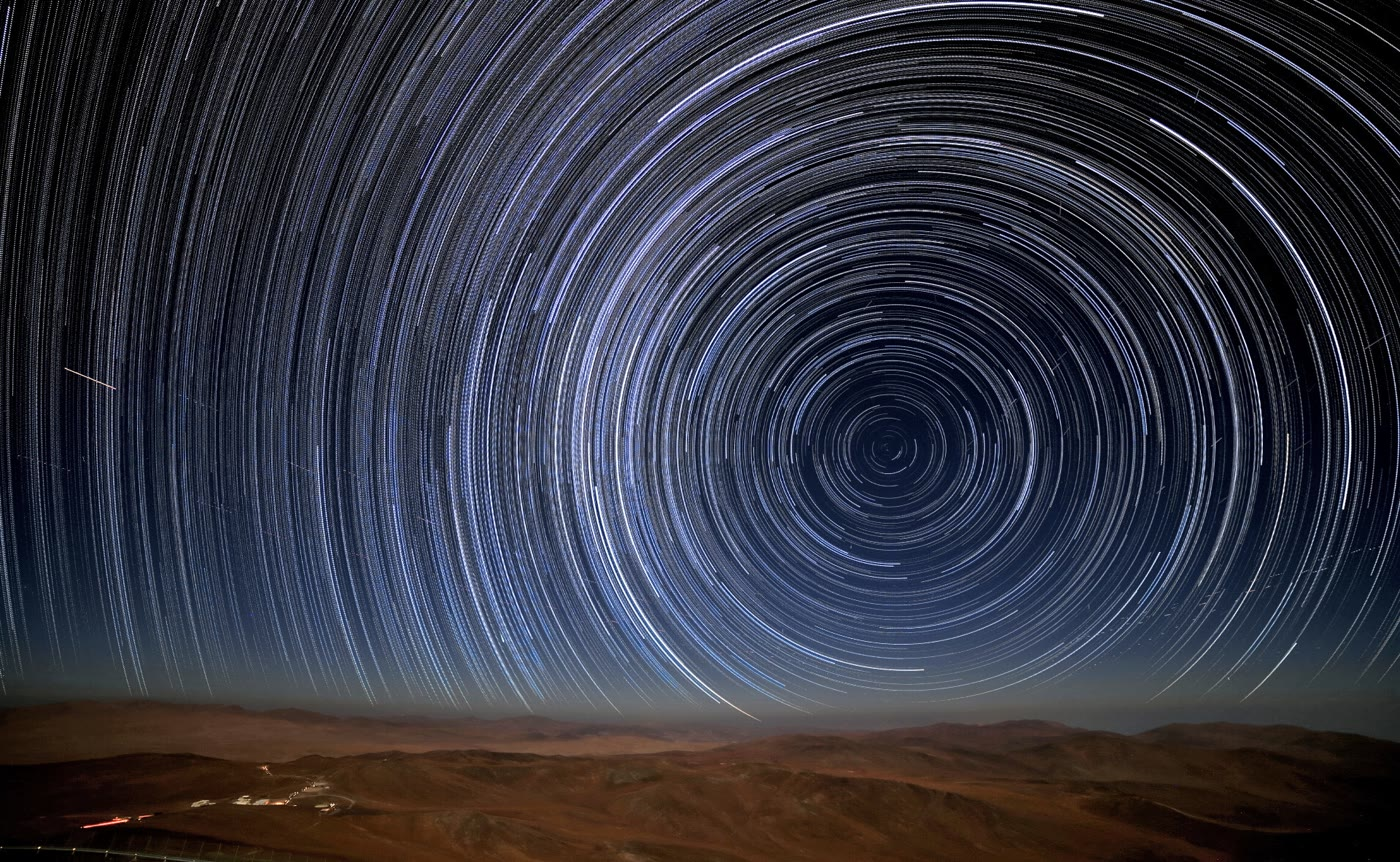
\includegraphics[width=0.8\linewidth]{images/book3/b1-star-trails-paranal.jpg}
% ledger: commons:eso-paranal-star-trails, mpc:paranal

{\small Rastros de estrelas sobre o Observatório do Paranal, no deserto do Atacama, na \omterm{def:b1:spherical-astronomy:geographic}{latitude} \ang{24.6} S: uma longa exposição registra o arco de cada estrela em torno do \omterm{def:b1:spherical-astronomy:celestial-sphere}{polo celeste} sul, que fica \ang{24.6} acima do horizonte sul. Fotografia de R.~Wesson/ESO, CC BY 4.0.}
\end{omfigure}

\section{Tempo sideral e tempo solar}

\begin{definition}[A eclíptica]\label{def:b1:spherical-astronomy:ecliptic}
A \emph{eclíptica}\index{eclíptica} é o \omterm{def:b1:spherical-astronomy:spherical-triangle}{círculo máximo} da \omterm{def:b1:spherical-astronomy:celestial-sphere}{esfera celeste} ao longo do qual o Sol parece se mover em um ano, o traço do plano da órbita da Terra. Ela é inclinada em relação ao \omterm{def:b1:spherical-astronomy:celestial-sphere}{equador celeste} pela \emph{obliquidade da eclíptica}\index{obliquidade da eclíptica} $\varepsilon$, a inclinação do eixo da Terra em relação à sua órbita. A eclíptica cruza o equador em dois pontos; o \emph{ponto vernal}\index{ponto vernal} $\gamma$ é aquele em que o Sol cruza o equador rumo ao norte, em março. A \omterm{def:b1:spherical-astronomy:geographic}{longitude} eclíptica $\lambda_\odot$ do Sol é o seu ângulo ao longo da eclíptica, a partir de $\gamma$, contado para leste.
\end{definition}

% ledger: earth:obliquity (23.44)
A obliquidade atual é $\varepsilon = \ang{23.44}$.

\begin{definition}[Tempo sideral]\label{def:b1:spherical-astronomy:sidereal-time}
O \emph{tempo sideral}\index{tempo sideral} local é o \omterm{def:b1:spherical-astronomy:equatorial}{ângulo horário} do \omterm{def:b1:spherical-astronomy:ecliptic}{ponto vernal} $\gamma$. Um dia sideral é o intervalo entre duas passagens de $\gamma$ pelo meridiano.
\end{definition}

Como a \omterm{def:b1:spherical-astronomy:equatorial}{ascensão reta} é contada para leste a partir de $\gamma$ e o \omterm{def:b1:spherical-astronomy:equatorial}{ângulo horário} para oeste a partir do meridiano, para qualquer estrela
\[
  H = \mathrm{LST} - \alpha ,
\]
em que LST é o \omterm{def:b1:spherical-astronomy:sidereal-time}{tempo sideral} local: uma estrela cruza o meridiano quando o \omterm{def:b1:spherical-astronomy:sidereal-time}{tempo sideral} é igual à sua \omterm{def:b1:spherical-astronomy:equatorial}{ascensão reta}. Um relógio de observatório que indica o \omterm{def:b1:spherical-astronomy:sidereal-time}{tempo sideral} mostra de relance qual parte do céu está acima da cabeça.

\begin{proposition}[Dias sideral e solar]\label{prop:b1:spherical-astronomy:sidereal-day}
Em um \omterm{def:b1:spherical-astronomy:tropical-year}{ano tropical} de $N$ dias solares médios, a Terra gira $N + 1$ vezes em relação às estrelas. Logo o dia sideral dura
\[
  \frac{N}{N + 1}\times\qty{24}{h},
\]
e com $N = 365.2422$ isso dá \qty{23}{h}~\qty{56}{min}~\qty{4.09}{s}: uma estrela cruza o meridiano \qty{3}{min}~\qty{56}{s} de \omterm{def:b1:spherical-astronomy:solar-time}{tempo solar médio} mais cedo a cada dia.
\end{proposition}

\begin{proof}
% ledger: usno:tropical-year, earth:Trot (23.9345 h)
Conte as voltas em relação ao Sol e em relação às estrelas ao longo de um ano. O Sol percorre uma vez a \omterm{def:b1:spherical-astronomy:ecliptic}{eclíptica} para leste em um ano, no sentido da rotação da Terra. Em relação ao Sol, a Terra dá portanto uma volta a menos do que em relação às estrelas: $N$ dias solares e $N + 1$ dias siderais preenchem o mesmo ano. O dia sideral é $N/(N+1)$ do dia solar, ou seja, $\qty{86400}{s}\times 365.2422/366.2422 = \qty{86164.09}{s}$; a diferença é $\qty{235.9}{s}$. Isso concorda com o período de rotação da Terra medido em relação às estrelas, \qty{23.9345}{h}.
\end{proof}

\begin{definition}[Tempo solar]\label{def:b1:spherical-astronomy:solar-time}
O \emph{tempo solar aparente}\index{tempo solar aparente} é o \omterm{def:b1:spherical-astronomy:equatorial}{ângulo horário} do Sol mais 12 horas: um relógio de sol o indica, e é meio-dia quando o Sol cruza o meridiano. O \emph{tempo solar médio}\index{tempo solar médio} é o \omterm{def:b1:spherical-astronomy:equatorial}{ângulo horário}, mais 12 horas, de um Sol médio fictício que percorre o \omterm{def:b1:spherical-astronomy:celestial-sphere}{equador celeste} com velocidade uniforme, completando uma volta em um \omterm{def:b1:spherical-astronomy:tropical-year}{ano tropical}. Sua diferença, aparente menos médio, é a \emph{equação do tempo}\index{equação do tempo}.
\end{definition}

O Sol verdadeiro adianta-se e atrasa-se em relação ao Sol médio por dois motivos. A Terra se move mais depressa perto do periélio, em início de janeiro, do que perto do afélio, de modo que o avanço do Sol ao longo da \omterm{def:b1:spherical-astronomy:ecliptic}{eclíptica} é irregular (segunda lei de Kepler); e o Sol se move ao longo da \omterm{def:b1:spherical-astronomy:ecliptic}{eclíptica}, que é inclinada em relação ao equador, de modo que até um movimento uniforme ao longo da \omterm{def:b1:spherical-astronomy:ecliptic}{eclíptica} se projeta sobre o equador (que é o que o \omterm{def:b1:spherical-astronomy:equatorial}{ângulo horário} mede) de maneira irregular, mais rápido perto dos solstícios do que perto dos equinócios. Os relógios civis marcam o \omterm{def:b1:spherical-astronomy:solar-time}{tempo solar médio} de um meridiano de referência de seu fuso horário; a hora média local na \omterm{def:b1:spherical-astronomy:geographic}{longitude} $\lambda$ está adiantada em relação à hora de Greenwich em $\lambda/\ang{15}$ horas.

\begin{omfigure}
\begin{tikzpicture}
\begin{axis}[omrecord, width=0.9\linewidth, height=5.2cm, xmin=0, xmax=365,
  xtick={0,31,59,90,120,151,181,212,243,273,304,334,365},
  xticklabels={J,F,M,A,M,J,J,A,S,O,N,D,},
  ylabel={equação do tempo (min)}, ymin=-20, ymax=21,
  tick label style={font=\scriptsize}, label style={font=\small}]
\addplot[black!50, line width=0.4pt] coordinates {(0,0) (365,0)};
\addplot[omDef, line width=1.1pt] table[x=day, y=eot_min] {figdata/out/bachelor-1-day_length-eot.dat};
\node[font=\scriptsize, above, fill=white, inner sep=1pt] at (axis cs:306,16.6) {$+16.4$};
\node[font=\scriptsize, below, fill=white, inner sep=1pt] at (axis cs:41,-14.4) {$-14.2$};
\end{axis}
\end{tikzpicture}

{\small A \omterm{def:b1:spherical-astronomy:solar-time}{equação do tempo} ao longo do ano (\omterm{def:b1:spherical-astronomy:solar-time}{tempo solar aparente} menos médio): um relógio de sol adianta-se até \qty{16.4}{min} em início de novembro e atrasa-se \qty{14.2}{min} em meados de fevereiro. Calculada a partir de uma órbita de Kepler com excentricidade 0,0167, obliquidade \ang{23.44}, a \omterm{def:b1:spherical-astronomy:geographic}{longitude} do periélio e a data do equinócio de março de 2026.}
% ledger: earth:ecc, earth:obliquity, nasa:earth-perihelion-longitude, usno:seasons-2026
\end{omfigure}

\section{Nascer e pôr do Sol}

\begin{proposition}[Nascer e pôr]\label{prop:b1:spherical-astronomy:rising}
Na \omterm{def:b1:spherical-astronomy:geographic}{latitude} $\varphi$, uma estrela de \omterm{def:b1:spherical-astronomy:equatorial}{declinação} $\delta$ que nasce e se põe cruza o horizonte nos \omterm{def:b1:spherical-astronomy:equatorial}{ângulos horários} $\pm H_0$, dados por
\[
  \cos H_0 = -\tan\varphi\tan\delta ,
\]
no \omterm{def:b1:spherical-astronomy:horizontal}{azimute} $\mathrm{A}_0$, com $\cos\mathrm{A}_0 = \sin\delta/\cos\varphi$ (no nascer; ela se põe em $\ang{360} - \mathrm{A}_0$). Ela permanece acima do horizonte durante $2H_0$, convertido em horas à razão de \ang{15} por hora.
\end{proposition}

\begin{proof}
No horizonte $h = 0$, e a \cref{prop:b1:spherical-astronomy:transform} dá $0 = \sin\varphi\sin\delta + \cos\varphi\cos\delta\cos H_0$, e $\cos\mathrm{A}_0 = \sin\delta/\cos\varphi$. O \omterm{def:b1:spherical-astronomy:equatorial}{ângulo horário} cresce uniformemente, de \ang{15} por hora, de $-H_0$ no nascer até $+H_0$ no pôr.
\end{proof}

Para o Sol, isso dá a duração do dia, se o Sol for tratado como um ponto e se a refração da luz pela atmosfera for ignorada (ambas as simplificações acrescentam alguns minutos de luz do dia). Nos equinócios $\delta = 0$, $H_0 = \ang{90}$: dia e noite duram doze horas em toda parte, e o Sol nasce exatamente a leste.

\begin{omfigure}
\begin{tikzpicture}
\begin{axis}[omrecord, width=0.85\linewidth, height=5.6cm, xmin=40, xmax=320, ymin=0, ymax=75,
  xtick={45,90,135,180,225,270,315}, xticklabels={NL,L,SL,S,SO,O,NO}, ytick={0,15,30,45,60,75},
  xlabel={azimute}, ylabel={altura do Sol ($^\circ$)},
  tick label style={font=\scriptsize}, label style={font=\small}]
\addplot[omThm, line width=1pt] table[x=az_deg, y=alt_deg] {figdata/out/bachelor-1-sun_paths-june.dat};
\addplot[black, line width=1pt] table[x=az_deg, y=alt_deg] {figdata/out/bachelor-1-sun_paths-equinox.dat};
\addplot[omDef, line width=1pt] table[x=az_deg, y=alt_deg] {figdata/out/bachelor-1-sun_paths-december.dat};
\begin{scope}[font=\scriptsize, fill=white, fill opacity=0.8, text opacity=1, inner sep=1pt]
  \node[omThm, above, fill=white] at (axis cs:180,68.4) {solstício de junho, $\ang{68.4}$};
  \node[above, fill=white] at (axis cs:180,45) {equinócios, $\ang{45}$};
  \node[omDef, above, fill=white] at (axis cs:180,21.6) {solstício de dezembro, $\ang{21.6}$};
\end{scope}
\end{axis}
\end{tikzpicture}

{\small O caminho do Sol pelo céu na \omterm{def:b1:spherical-astronomy:geographic}{latitude} \ang{45} N no solstício de junho (em vermelho), nos equinócios (em preto) e no solstício de dezembro (em azul), com as \omterm{def:b1:spherical-astronomy:horizontal}{alturas angulares} ao meio-dia $\ang{90} - \varphi + \delta_\odot$. Nos equinócios o Sol nasce exatamente a leste e se põe exatamente a oeste; em junho ele nasce a nordeste.}
\end{omfigure}

\begin{proposition}[Declinação do Sol]\label{prop:b1:spherical-astronomy:sun-declination}
Quando o Sol está na \omterm{def:b1:spherical-astronomy:geographic}{longitude} \omterm{def:b1:spherical-astronomy:ecliptic}{eclíptica} $\lambda_\odot$, sua \omterm{def:b1:spherical-astronomy:equatorial}{declinação} e sua \omterm{def:b1:spherical-astronomy:equatorial}{ascensão reta} satisfazem
\[
  \sin\delta_\odot = \sin\varepsilon\sin\lambda_\odot, \qquad
  \tan\alpha_\odot = \cos\varepsilon\tan\lambda_\odot .
\]
\end{proposition}

\begin{proof}
Tome eixos com $x$ apontando para $\gamma$ e $z$ para o \omterm{def:b1:spherical-astronomy:celestial-sphere}{polo celeste} norte. Nos eixos $x$, $y'$, $z'$ ligados à \omterm{def:b1:spherical-astronomy:ecliptic}{eclíptica}, com $z'$ apontando para o seu polo, a direção do Sol é $(\cos\lambda_\odot, \sin\lambda_\odot, 0)$. Os eixos da \omterm{def:b1:spherical-astronomy:ecliptic}{eclíptica} são os do equador girados pelo ângulo $\varepsilon$ em torno de $x$, de modo que, nos eixos equatoriais, a direção do Sol é
$(\cos\lambda_\odot,\ \sin\lambda_\odot\cos\varepsilon,\
\sin\lambda_\odot\sin\varepsilon)$. Sua componente $z$ é $\sin\delta_\odot$; a razão entre suas componentes $y$ e $x$ é $\tan\alpha_\odot$.
\end{proof}

\begin{omfigure}
\begin{tikzpicture}
\begin{axis}[omrecord, width=0.9\linewidth, height=6cm, xmin=0, xmax=365, ymin=0, ymax=24,
  xtick={0,31,59,90,120,151,181,212,243,273,304,334,365},
  xticklabels={J,F,M,A,M,J,J,A,S,O,N,D,}, ytick={0,6,12,18,24},
  ylabel={duração do dia (h)}, tick label style={font=\scriptsize}, label style={font=\small},
  legend style={font=\scriptsize, at={(0.5,1.02)}, anchor=south, draw=none}, legend columns=5,
  legend cell align=left]
\addplot[black, line width=0.9pt] table[x=day, y=lat0] {figdata/out/bachelor-1-day_length-lengths.dat};
\addplot[omDef, line width=0.9pt] table[x=day, y=lat30] {figdata/out/bachelor-1-day_length-lengths.dat};
\addplot[omThm, line width=0.9pt] table[x=day, y=lat45] {figdata/out/bachelor-1-day_length-lengths.dat};
\addplot[omField, line width=0.9pt] table[x=day, y=lat60] {figdata/out/bachelor-1-day_length-lengths.dat};
\addplot[black, line width=0.9pt, densely dashed] table[x=day, y=lat70] {figdata/out/bachelor-1-day_length-lengths.dat};
\legend{\ang{0}, \ang{30} N, \ang{45} N, \ang{60} N, \ang{70} N}
\end{axis}
\end{tikzpicture}

{\small Duração do dia (com o centro do Sol acima do horizonte geométrico) ao longo do ano em cinco \omterm{def:b1:spherical-astronomy:geographic}{latitudes} do hemisfério norte, com base nas
\cref{prop:b1:spherical-astronomy:rising,prop:b1:spherical-astronomy:sun-declination}.
\ang{70} N o Sol permanece acima do horizonte durante semanas em torno do solstício de junho e fica abaixo dele em torno do solstício de dezembro. No hemisfério sul as curvas estão deslocadas de meio ano.}
\end{omfigure}

\begin{definition}[Insolação]\label{def:b1:spherical-astronomy:insolation}
A \emph{insolação}\index{insolação} em um lugar e em um instante é a potência da luz solar recebida por unidade de área de uma superfície horizontal no topo da atmosfera. Sendo $S_0$ a irradiância solar à distância média $a$ do Sol, $r$ a distância real e $\theta_z$ a distância zenital do Sol,
\[
  I = S_0\left(\frac{a}{r}\right)^{2}\cos\theta_z = S_0\left(\frac{a}{r}\right)^{2}\sin h_\odot
  \quad (h_\odot > 0), \qquad I = 0 \text{ à noite}.
\]
\end{definition}

% ledger: earth:TSI (1361 W/m2), earth:peri, earth:aph, earth:a
O fator $(a/r)^2$ é a lei do inverso do quadrado para a luz (nos livros de física); o fator $\cos\theta_z$ aparece porque um feixe de seção transversal de um metro quadrado se espalha por $1/\cos\theta_z$ metros quadrados de solo horizontal. Com
$S_0 = \qty{1361}{W.m^{-2}}$ e uma distância Sol--Terra entre \qty{147.1e6}{km} no periélio e \qty{152.1e6}{km} no afélio, o fator $(a/r)^2$ varia $\pm\qty{3.4}{\percent}$ ao longo do ano. A
inclinação do eixo faz bem mais: altera tanto a \omterm{def:b1:spherical-astronomy:horizontal}{altura angular} do Sol ao meio-dia quanto a duração do dia, e esses dois efeitos juntos produzem as estações. As somas diárias e anuais da \omterm{def:b1:spherical-astronomy:insolation}{insolação}, que movem o clima, são calculadas em
\cref{ch:b1:radiation-heat-transport}.


\section{Calendários}

\begin{definition}[Ano tropical]\label{def:b1:spherical-astronomy:tropical-year}
O \emph{ano tropical}\index{ano tropical} é o intervalo médio entre duas passagens do Sol pelo \omterm{def:b1:spherical-astronomy:ecliptic}{ponto vernal}. Ele governa as estações; dura 365.2422 dias solares médios.
\end{definition}

% ledger: usno:tropical-year, earth:Psid (365.256 d)
O \omterm{def:b1:spherical-astronomy:tropical-year}{ano tropical} é cerca de vinte minutos mais curto que o ano sideral, o tempo que a Terra leva para voltar ao mesmo lugar entre as estrelas (365.256 dias), porque o eixo da Terra gira lentamente --- ele precessiona --- e leva o \omterm{def:b1:spherical-astronomy:ecliptic}{ponto vernal} para trás ao longo da \omterm{def:b1:spherical-astronomy:ecliptic}{eclíptica} (no Livro 4). Um calendário precisa ajustar um número inteiro de dias ao \omterm{def:b1:spherical-astronomy:tropical-year}{ano tropical}, para que as estações voltem nas mesmas datas.

\begin{proposition}[O ano gregoriano]\label{prop:b1:spherical-astronomy:gregorian}
No calendário gregoriano, um ano é bissexto, com 366 dias, se seu número é divisível por 4, exceto os anos-século, que são bissextos apenas se forem divisíveis por 400. Seu ano médio é
\[
  365 + \frac14 - \frac1{100} + \frac1{400} = \num{365.2425}\text{ dias},
\]
e ele se desloca em relação às estações um dia a cada cerca de 3300 anos.
\end{proposition}

\begin{proof}
% ledger: usno:leap-rule, usno:tropical-year
Em 400 anos há 100 anos divisíveis por 4; entre eles há quatro anos-século, dos quais três não são divisíveis por 400. Há portanto 97 anos bissextos e $400\times 365 + 97 = 146\,097$ dias, ou seja, 365.2425 dias por ano. Frente a um \omterm{def:b1:spherical-astronomy:tropical-year}{ano tropical} de 365.2422 dias, o excesso é de 0.0003 dia por ano: um dia em $1/0.0003 \approx 3300$ anos.
\end{proof}

\begin{history}[A reforma de 1582]
% ledger: usno:gregorian-1582
O calendário juliano, herdado de Roma, acrescentava um dia bissexto a cada quatro anos: seu ano de 365.25 dias é mais longo que o \omterm{def:b1:spherical-astronomy:tropical-year}{ano tropical} em 0.0078 dia, ou seja, um dia a cada 128 anos. Ao longo dos séculos a data do equinócio de março afastou-se de 21 de março, data em que se baseava o cálculo da Páscoa. Em 1582 o papa Gregório~XIII introduziu o calendário que leva seu nome, que eliminou de uma vez os dias acumulados e substituiu a regra juliana pela regra de \cref{prop:b1:spherical-astronomy:gregorian}. Ele se tornou o calendário civil aceito internacionalmente.
\end{history}

\begin{inthefield}[Localizar uma posição pelas estrelas]
Antes da localização por satélite, os navegadores no mar encontravam sua \omterm{def:b1:spherical-astronomy:geographic}{latitude} e \omterm{def:b1:spherical-astronomy:geographic}{longitude} pelo céu. Com um sextante mediam a \omterm{def:b1:spherical-astronomy:horizontal}{altura angular} do Sol ao meio-dia, ou a de duas ou três estrelas ao entardecer, e liam a hora num cronômetro ajustado à hora do meridiano de Greenwich. Cada \omterm{def:b1:spherical-astronomy:horizontal}{altura angular}, junto com a \omterm{def:b1:spherical-astronomy:equatorial}{declinação} da estrela e seu \omterm{def:b1:spherical-astronomy:equatorial}{ângulo horário} em Greenwich, tirados de um almanaque, dá um pequeno círculo sobre a Terra no qual está o navio: o círculo dos pontos em que a estrela tem aquela \omterm{def:b1:spherical-astronomy:horizontal}{altura angular}. Dois ou três desses círculos se cruzam na posição do navio --- trigonometria esférica resolvida no mar todos os dias. A \omterm{def:b1:spherical-astronomy:horizontal}{altura angular} do Sol ao meio-dia sozinha dá a \omterm{def:b1:spherical-astronomy:geographic}{latitude}
(\cref{prop:b1:spherical-astronomy:culmination}); a hora do meio-dia local no relógio dá a \omterm{def:b1:spherical-astronomy:geographic}{longitude}, à razão de quatro minutos de tempo por grau.
\begin{center}
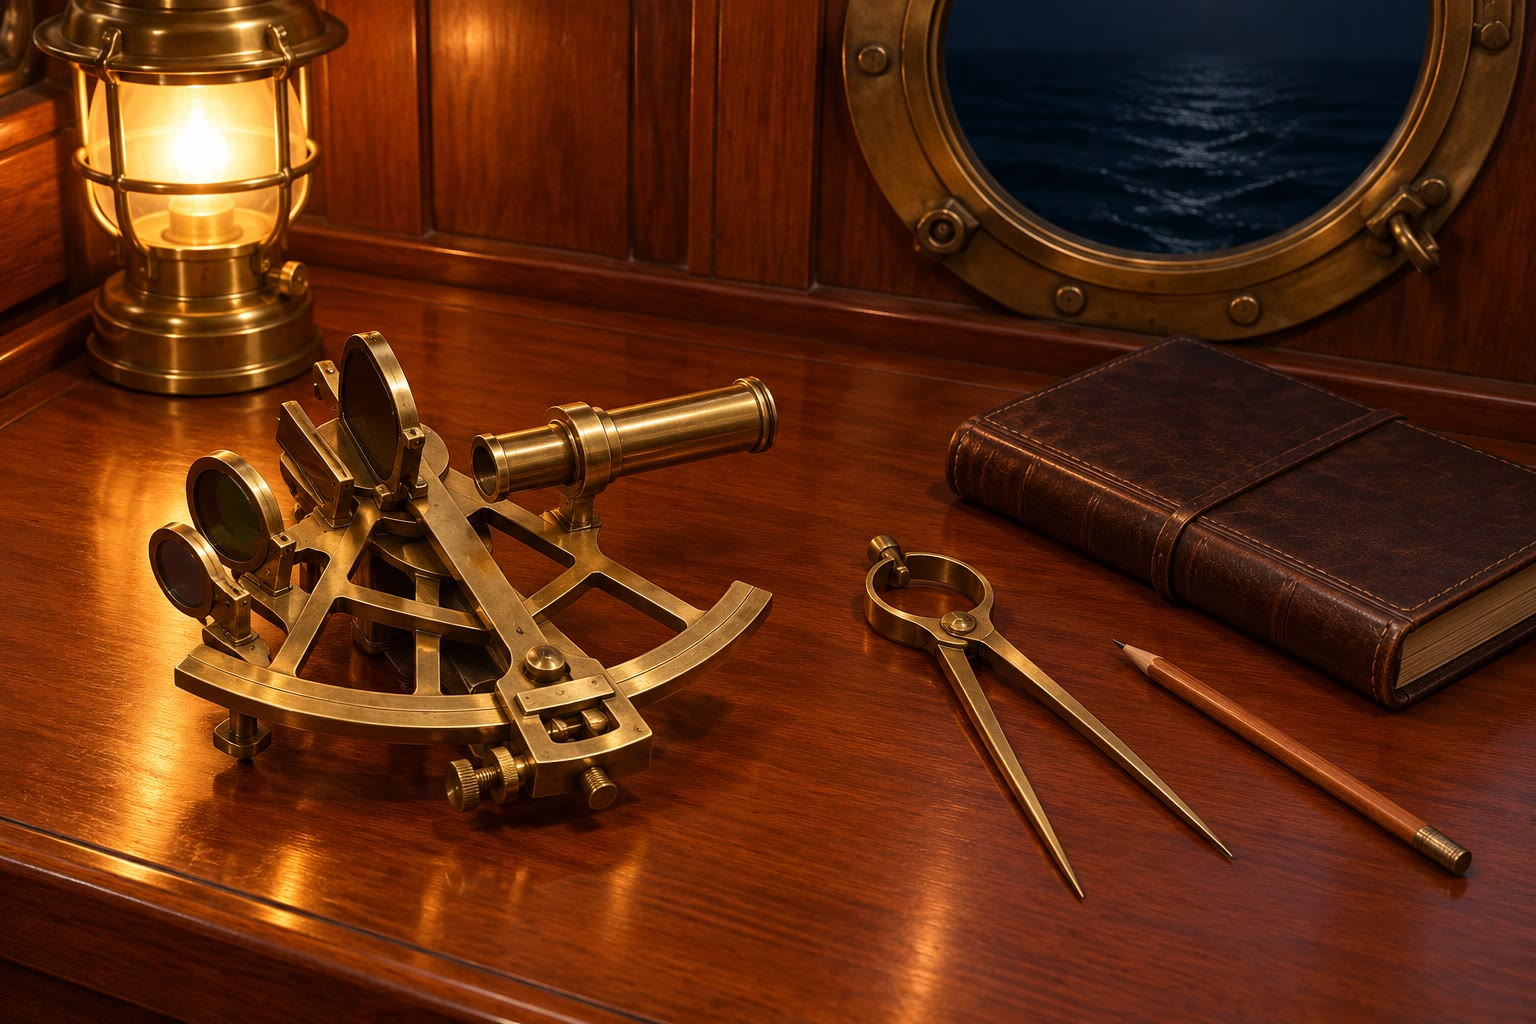
\includegraphics[width=0.55\linewidth]{images/book3/ai/b1-sextant.jpg}
\end{center}
\end{inthefield}

\section{Exercícios}

\begin{exercise}[$\star$]\label{exo:b1:spherical-astronomy:1}
Um observador está na \omterm{def:b1:spherical-astronomy:geographic}{latitude} \ang{52} N. Calcule a \omterm{def:b1:spherical-astronomy:horizontal}{altura angular} do \omterm{def:b1:spherical-astronomy:celestial-sphere}{polo celeste} norte acima do horizonte. Quais estrelas, pela sua \omterm{def:b1:spherical-astronomy:equatorial}{declinação}, nunca se põem ali, e quais nunca nascem?
\end{exercise}

\begin{exercise}[$\star$]\label{exo:b1:spherical-astronomy:2}
Converta uma \omterm{def:b1:spherical-astronomy:equatorial}{ascensão reta} de \qty{6}{h}~\qty{45}{min} em graus. Com um \omterm{def:b1:spherical-astronomy:sidereal-time}{tempo sideral} local de \qty{10}{h}~\qty{0}{min}, calcule o \omterm{def:b1:spherical-astronomy:equatorial}{ângulo horário} de uma estrela com essa \omterm{def:b1:spherical-astronomy:equatorial}{ascensão reta}. Ela está a leste ou a oeste do meridiano?
\end{exercise}

\begin{exercise}[$\star$]\label{exo:b1:spherical-astronomy:3}
Na \omterm{def:b1:spherical-astronomy:geographic}{latitude} \ang{40} N, calcule a \omterm{def:b1:spherical-astronomy:horizontal}{altura angular} do Sol ao meio-dia nos dois solstícios e nos equinócios ($\varepsilon = \ang{23.44}$).
\end{exercise}

\begin{exercise}[$\star$]\label{exo:b1:spherical-astronomy:4}
1900 foi um ano bissexto? E 2000? Será 2100? Calcule de quantos dias por século o calendário juliano se desloca em relação a um \omterm{def:b1:spherical-astronomy:tropical-year}{ano tropical} de 365.2422 dias, e de quantos o calendário gregoriano se desloca.
\end{exercise}

\begin{exercise}[$\star\star$]\label{exo:b1:spherical-astronomy:5}
Dois pontos estão na \omterm{def:b1:spherical-astronomy:geographic}{latitude} \ang{45} N, nas \omterm{def:b1:spherical-astronomy:geographic}{longitudes} \ang{0} e \ang{90} L. Calcule a distância sobre o \omterm{def:b1:spherical-astronomy:spherical-triangle}{círculo máximo} entre eles ($R = \qty{6371}{km}$) e a distância ao longo de seu paralelo. Qual é a menor, e por quanto?
\end{exercise}

\begin{exercise}[$\star\star$]\label{exo:b1:spherical-astronomy:6}
Na \omterm{def:b1:spherical-astronomy:geographic}{latitude} \ang{48} N, uma estrela de \omterm{def:b1:spherical-astronomy:equatorial}{declinação} \ang{20} tem \omterm{def:b1:spherical-astronomy:equatorial}{ângulo horário} \ang{30}. Calcule sua \omterm{def:b1:spherical-astronomy:horizontal}{altura angular} e seu \omterm{def:b1:spherical-astronomy:horizontal}{azimute}. Em que direção o observador deve olhar?
\end{exercise}

\begin{exercise}[$\star\star$]\label{exo:b1:spherical-astronomy:7}
Calcule a duração do dia na \omterm{def:b1:spherical-astronomy:geographic}{latitude} \ang{60} N no solstício de junho, tratando o Sol como um ponto sobre um horizonte geométrico. Confira sua resposta na figura da duração do dia.
\end{exercise}

\begin{exercise}[$\star\star$]\label{exo:b1:spherical-astronomy:8}
Uma estrela cruza o meridiano nesta noite às 22 h, no \omterm{def:b1:spherical-astronomy:solar-time}{tempo solar médio} local. Calcule em que hora ela cruzará o meridiano daqui a 30 dias. Em quantos dias ela cruzará ao meio-dia, invisível na luz do dia?
\end{exercise}

\begin{exercise}[$\star\star$]\label{exo:b1:spherical-astronomy:9}
Calcule a \omterm{def:b1:spherical-astronomy:insolation}{insolação} no topo da atmosfera ao meio-dia na \omterm{def:b1:spherical-astronomy:geographic}{latitude} \ang{45} N (a) em um equinócio, tomando $r = a$; (b) no solstício de junho, tomando para $r$ a distância do afélio. Dados: $S_0 = \qty{1361}{W.m^{-2}}$, $a = \qty{149.598e6}{km}$, afélio \qty{152.100e6}{km}.
\end{exercise}

\begin{exercise}[$\star\star\star$]\label{exo:b1:spherical-astronomy:10}
Usando \cref{prop:b1:spherical-astronomy:sun-declination}, calcule a \omterm{def:b1:spherical-astronomy:equatorial}{declinação} e a \omterm{def:b1:spherical-astronomy:equatorial}{ascensão reta} do Sol quando sua \omterm{def:b1:spherical-astronomy:geographic}{longitude} \omterm{def:b1:spherical-astronomy:ecliptic}{eclíptica} é \ang{60}. De quantos graus a \omterm{def:b1:spherical-astronomy:equatorial}{ascensão reta} fica atrás da \omterm{def:b1:spherical-astronomy:geographic}{longitude}? Explique, com esse resultado, por que a inclinação da \omterm{def:b1:spherical-astronomy:ecliptic}{eclíptica} contribui para a \omterm{def:b1:spherical-astronomy:solar-time}{equação do tempo}.
\end{exercise}

\begin{exercise}[$\star\star\star$]\label{exo:b1:spherical-astronomy:11}
Mostre que no solstício de junho o Sol nasce no \omterm{def:b1:spherical-astronomy:horizontal}{azimute} $\mathrm{A}_0$, com $\cos\mathrm{A}_0 = \sin\varepsilon/\cos\varphi$. Em que \omterm{def:b1:spherical-astronomy:geographic}{latitude} ele nasce exatamente a nordeste? O que acontece com a fórmula nas \omterm{def:b1:spherical-astronomy:geographic}{latitudes} acima de $\ang{90} - \varepsilon$?
\end{exercise}

\begin{exercise}[$\star\star\star$]\label{exo:b1:spherical-astronomy:12}
Um fuso esférico é a parte de uma esfera entre dois semicírculos máximos que unem dois pontos opostos, formando entre si o ângulo $\theta$. (a) Mostre que sua área é $2\theta R^2$. (b) Cada lado de um \omterm{def:b1:spherical-astronomy:spherical-triangle}{triângulo esférico} $ABC$, prolongado até um \omterm{def:b1:spherical-astronomy:spherical-triangle}{círculo máximo} completo, determina com os outros dois lados três pares de fusos opostos, de ângulos $A$, $B$, $C$, que cobrem a esfera; o triângulo e o seu oposto são cobertos três vezes. Deduza o teorema de Girard: a área do triângulo é $R^2(A + B + C - \pi)$. (c) Aplique-o ao triângulo com três ângulos retos e ao triângulo desenhado neste capítulo (ângulos \ang{89.9}, \ang{64.9}, \ang{67.4}).
\end{exercise}

\section{Problema: uma noite em um observatório de montanha}

\begin{problem}[{Problema de fim de semana --- onde se situa o Observatório do Paranal, o que mostra o seu céu e quanto dura a sua noite mais longa}]
\label{pb:b1:spherical-astronomy:1}
% ledger: mpc:paranal, mpc:greenwich, simbad:sirius, simbad:canopus, usno:seasons-2026, earth:obliquity, usno:tropical-year
% numbers computed in the scratch calculator calc/ch01.py from the rounded data
O Observatório do Paranal fica no deserto do Atacama, na \omterm{def:b1:spherical-astronomy:geographic}{latitude} \ang{24.63} S, \omterm{def:b1:spherical-astronomy:geographic}{longitude} \ang{70.40} O. O Observatório Real de Greenwich, a partir do qual se contam as \omterm{def:b1:spherical-astronomy:geographic}{longitudes}, fica em \ang{51.48} N, \ang{0.00}. Duas estrelas brilhantes do céu do sul têm as coordenadas
\begin{center}
\small
\begin{tabular}{lcc}
\hline
estrela & \omterm{def:b1:spherical-astronomy:equatorial}{ascensão reta} & \omterm{def:b1:spherical-astronomy:equatorial}{declinação} \\
\hline
Sirius & \qty{6}{h}~\qty{45}{min}~\qty{9}{s} & \ang{-16.72} \\
Canopus & \qty{6}{h}~\qty{23}{min}~\qty{57}{s} & \ang{-52.70} \\
\hline
\end{tabular}
\end{center}
Use $R = \qty{6371}{km}$, $\varepsilon = \ang{23.44}$, um \omterm{def:b1:spherical-astronomy:tropical-year}{ano tropical} de 365.2422 dias, e trate o Sol como um ponto sobre um horizonte geométrico.

\medskip
\noindent\textbf{Parte I --- O Paranal no globo.}
\begin{enumerate}
  \item Dê as colatitudes do Paranal e de Greenwich, e a diferença de \omterm{def:b1:spherical-astronomy:geographic}{longitude} entre eles.
  \item Escreva a lei dos cossenos para o triângulo Polo Norte--Paranal--Greenwich e calcule o cosseno da distância angular $\Delta$ entre os dois observatórios.
  \item Deduza $\Delta$ em graus e a distância sobre o \omterm{def:b1:spherical-astronomy:spherical-triangle}{círculo máximo}, em quilômetros.
  \item Calcule o rumo inicial do Paranal em direção a Greenwich
        (\cref{met:b1:spherical-astronomy:great-circle}).
  \item Confira o rumo pela lei dos senos.
  \item Uma aeronave que mantivesse esse rumo durante todo o trajeto chegaria a Greenwich? Explique.
\end{enumerate}

\medskip
\noindent\textbf{Parte II --- O céu do Paranal.}
\begin{enumerate}[resume]
  \item Calcule a \omterm{def:b1:spherical-astronomy:horizontal}{altura angular} do \omterm{def:b1:spherical-astronomy:celestial-sphere}{polo celeste} sul acima do horizonte sul do Paranal.
  \item Calcule a \omterm{def:b1:spherical-astronomy:horizontal}{altura angular} em que Sirius cruza o meridiano e de que lado do \omterm{def:b1:spherical-astronomy:celestial-sphere}{zênite} ela fica.
  \item Determine a declinação-limite abaixo da qual uma estrela é circumpolar no Paranal. Canopus é circumpolar?
  \item Calcule a maior \omterm{def:b1:spherical-astronomy:horizontal}{altura angular} que Canopus atinge.
  \item Calcule o \omterm{def:b1:spherical-astronomy:equatorial}{ângulo horário} em que Sirius nasce e por quanto tempo ela permanece acima do horizonte, em horas siderais.
  \item Calcule o \omterm{def:b1:spherical-astronomy:horizontal}{azimute} em que Sirius nasce.
\end{enumerate}

\medskip
\noindent\textbf{Parte III --- Relógios.}
\begin{enumerate}[resume]
  \item Qual é o \omterm{def:b1:spherical-astronomy:sidereal-time}{tempo sideral} local quando Sirius cruza o meridiano?
  \item Calcule a duração do dia sideral e de quantos minutos a passagem de uma estrela pelo meridiano se adianta a cada noite.
  \item Tome o \omterm{def:b1:spherical-astronomy:sidereal-time}{tempo sideral} local à meia-noite média local como sendo \qty{12}{h} no equinócio de março (20 de março de 2026), quando o Sol está perto do \omterm{def:b1:spherical-astronomy:ecliptic}{ponto vernal}; ele então ganha $24/365.2422$ horas por dia. Quantos dias depois do equinócio Sirius cruza o meridiano à meia-noite média local? Em que data?
  \item Nessa noite, em quanto o tempo médio local do Paranal difere do tempo de Greenwich?
  \item A \omterm{def:b1:spherical-astronomy:solar-time}{equação do tempo} é então de cerca de \qty{-3}{min}. Que horas marca um relógio de sol no observatório (\omterm{def:b1:spherical-astronomy:solar-time}{tempo solar aparente}) quando Sirius cruza o meridiano?
  \item Calcule quanto antes ela cruza o meridiano uma semana depois.
\end{enumerate}

\noindent\textbf{Parte IV --- A noite mais longa.}
\begin{enumerate}[resume]
  \item Calcule a \omterm{def:b1:spherical-astronomy:equatorial}{declinação} do Sol em cada solstício.
  \item Calcule a \omterm{def:b1:spherical-astronomy:horizontal}{altura angular} do Sol ao meio-dia no Paranal nos solstícios de junho e de dezembro. De que lado do \omterm{def:b1:spherical-astronomy:celestial-sphere}{zênite} ele fica em dezembro?
  \item No solstício de dezembro, a distância Sol--Terra é 0.9837 vez a distância média. Calcule a \omterm{def:b1:spherical-astronomy:insolation}{insolação} ao meio-dia no topo da atmosfera acima do Paranal ($S_0 = \qty{1361}{W.m^{-2}}$).
  \item Em qual solstício a noite é mais longa no Paranal? Calcule o \omterm{def:b1:spherical-astronomy:equatorial}{ângulo horário} do pôr do Sol nessa data.
  \item Em que \omterm{def:b1:spherical-astronomy:horizontal}{azimute} o Sol nasce nessa data?
  \item Deduza a duração da noite mais longa do ano no Paranal, em horas e minutos.
\end{enumerate}
\end{problem}
